% Author: Izaak Neutelings (October 2020)
% https://mathworld.wolfram.com/PhasePortrait.html
\documentclass[border=3pt,tikz]{standalone}
\usepackage{amsmath} % for \dfrac
\usepackage{physics,siunitx}
\usepackage{tikz,pgfplots}
\usepackage[outline]{contour} % glow around text
\contourlength{1.0pt}
\usetikzlibrary{angles,quotes} % for pic (angle labels)
\usetikzlibrary{arrows.meta}
\usetikzlibrary{decorations.markings}
%\usetikzlibrary{bending} % for arrow head angle
\tikzset{>=latex} % for LaTeX arrow head
\usepackage{xcolor}

\colorlet{xcol}{blue!60!black}
\colorlet{myred}{red!80!black}
\colorlet{myblue}{blue!80!black}
\colorlet{mygreen}{green!40!black}
\colorlet{myorange}{orange!90!black}
\colorlet{mypurple}{red!50!blue!90!black!80}
\colorlet{mydarkred}{myred!80!black}
\colorlet{mydarkblue}{myblue!80!black}
\tikzstyle{xline}=[xcol,thick]
\tikzstyle{width}=[{Latex[length=5,width=3]}-{Latex[length=5,width=3]},thick]
\tikzset{
  traj/.style 2 args={xline,postaction={decorate},decoration={markings,
    mark=at position #1 with {\arrow{<}},
    mark=at position #2 with {\arrow{<}}}
  }
}
\def\tick#1#2{\draw[thick] (#1)++(#2:0.12) --++ (#2-180:0.24)}
\def\N{100} % number of samples


\begin{document}


% CIRCLE on axis
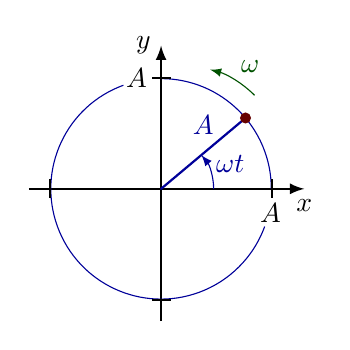
\begin{tikzpicture}
    \def\A{1.4}
    \def\ang{40}
    \coordinate (O) at (0,0);
    \coordinate (X) at (\A,0);
    \coordinate (R) at (\ang:\A);
    \draw[->,thick] (-1.2*\A,0) -- (1.3*\A,0) node[below] {$x$};
    \draw[->,thick] (0,-1.2*\A) -- (0,1.3*\A) node[left] {$y$};
    \node[inner sep=2] (R') at (R) {};
    \draw[xcol] (0:\A) arc(0:90:\A);
    \draw[xcol] (110:\A) arc(110:340:\A);
    \draw[xcol,thick,line cap=round] (O) -- (R) node[midway,above=3] {$A$};
    \tick{0,-\A-0.008}{0}; %node[left=-1,scale=1] {$A$};
    \tick{0, \A+0.008}{0} node[left=-2,scale=1] {$A$};
    \tick{-\A-0.008,0}{90}; %node[below=-1,scale=1] {$A$};
    \tick{ \A+0.008,0}{90} node[left=0.5,below=-2,scale=1] {$A$};
    \draw pic[->,"$\omega t$",xcol,draw=xcol,angle radius=19,angle eccentricity=1.4] {angle=X--O--R};
    \fill[myred!50!black] (R) circle (0.07);
    \draw[->,mygreen!80!black] (\ang+5:1.2*\A) arc(\ang+5:\ang+35:0.9*\A) node[midway,above right=-1] {$\omega$};
\end{tikzpicture}


% CIRCLE on axis + phase
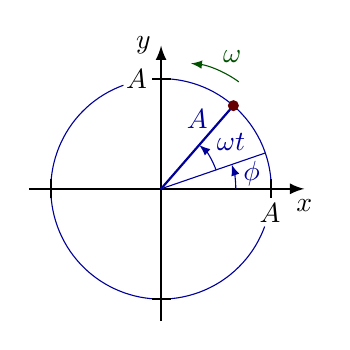
\begin{tikzpicture}
    \def\A{1.4}
    \def\ang{30}
    \def\phase{19}
    \coordinate (O) at (0,0);
    \coordinate (X) at (\A,0);
    \coordinate (R0) at (\phase:\A);
    \coordinate (R) at (\ang+\phase:\A);
    \draw[->,thick] (-1.2*\A,0) -- (1.3*\A,0) node[below] {$x$};
    \draw[->,thick] (0,-1.2*\A) -- (0,1.3*\A) node[left] {$y$};
    \node[inner sep=2] (R') at (R) {};
    \draw[xcol] (0:\A) arc(0:90:\A);
    \draw[xcol] (110:\A) arc(110:340:\A);
    \draw[xcol,thick,line cap=round] (O) -- (R) node[midway,above=3] {$A$};
    \draw[xcol,thin] (O) -- (R0);
    \tick{0,-\A}{0}; %node[left=-1,scale=1] {$A$};
    \tick{0, \A}{0} node[left=-2,scale=1] {$A$};
    \tick{-\A,0}{90}; %node[below=-1,scale=1] {$A$};
    \tick{ \A,0}{90} node[left=0.5,below=-2,scale=1] {$A$};
    \draw pic[->,"$\phi$",xcol,draw=xcol,angle radius=27,angle eccentricity=1.23] {angle=X--O--R0};
    \draw pic[->,"$\omega t$",xcol,draw=xcol,angle radius=21,angle eccentricity=1.45] {angle=R0--O--R};
    \fill[myred!50!black] (R) circle (0.07);
    \draw[->,mygreen!80!black] (\ang+\phase+5:1.2*\A) arc(\ang+\phase+5:\ang+\phase+35:0.9*\A) node[midway,above right=-1] {$\omega$};
\end{tikzpicture}


% COS
\def\xmax{6.6} % max x axis
\def\ymax{1.2} % max y axis
\def\A{0.8}    % amplitude
\def\om{(2.55*360/(0.94*\xmax))} % angular frequency in degrees
\begin{tikzpicture}

    % AXIS
    \draw[->,thick] (0,-\ymax) -- (0,\ymax) node[left,xcol] {$x$};
    \draw[->,thick] (-0.2*\ymax,0) -- (\xmax,0) node[below] {$t$};
    \draw[dashed] ({360/\om},1.2*\A) --++ (0,-2.7*\A);
    \tick{0,\A}{0} node[left=-1,scale=0.9] {$A$};
    \tick{{360/\om},0}{90} node[below,scale=0.9] {\contour{white}{$T$}};
    \tick{{720/\om},0}{90} node[below,scale=0.9] {$2T$};
    \draw[<->]
    (0,-1.35*\A) --++ ({360/\om},0)
    node[midway,fill=white,inner sep=1,scale=0.9] {$T = 2\pi/\omega$};

    % PLOT
    \draw[xline,samples=\N,smooth,variable=\x,domain=0:0.94*\xmax]
    plot(\x,{\A*cos(\om*\x)});
    %\node[xcol,above=2,right=4] at ({720/\om},\A) {$x(t)=A\cos(\omega t)$};

\end{tikzpicture}


% COS - phase
\begin{tikzpicture}
    \def\phase{60}

    % AXIS
    \draw[->,thick] (0,-\ymax) -- (0,\ymax) node[left,xcol] {$x$};
    \draw[->,thick] (-0.2*\ymax,0) -- (\xmax,0) node[below] {$t$};
    \tick{0,\A}{0} node[left=-1,scale=0.9] {$A$};
    \tick{{\phase/\om},0}{90} node[below,scale=0.9] {$t_0$};
    \draw[dashed] ({\phase/\om},0) --++ (0,1.2*\A);
    \draw[dashed] ({180/\om},-1.3*\A) --++ (0,1.5*\A);
    \draw[dashed] ({(180+\phase)/\om},-1.3*\A) --++ (0,1.5*\A);
    \draw[->]
    ({180/\om},-1.25*\A) --++ ({\phase/\om},0)
    node[midway,below,scale=0.9] {$t_0 = \phi/\omega$};

    % PLOT
    \draw[xcol!30,thin,dashed,samples=\N,smooth,variable=\x,domain=0:0.94*\xmax]
    plot(\x,{\A*cos(\om*\x)});
    \draw[xline,samples=\N,smooth,variable=\x,domain=0:0.94*\xmax]
    plot(\x,{\A*cos(\om*\x-\phase)});
    \tick{{(360+\phase)/\om},0}{90} node[below,scale=0.9] {\contour{white}{$t_0+T$}};
    \tick{{(720+\phase)/\om},0}{90} node[below,scale=0.9] {\contour{white}{$t_0+2T$}};

\end{tikzpicture}


% COS - phase - vertical shift
\begin{tikzpicture}
    \def\phase{60}
    \def\C{0.5*\A}

    % AXIS
    \draw[->,thick] (0,\C-\ymax) -- (0,\C+1.05*\ymax) node[left,xcol] {$y$};
    \draw[->,thick] (-0.2*\ymax,0) -- (\xmax,0) node[below] {$t$};
    \tick{0,\C+\A}{0} node[left=-1,scale=0.9] {$A+y_0$};
    \tick{0,\C-\A}{0} node[left=-1,scale=0.9] {$-A+y_0$};
    \tick{0,\C}{0} node[left=-1,scale=0.9] {$y_0$};

    % PLOT
    \draw[dashed] (0,\C) --++ (0.95*\xmax,0);
    \draw[xline,samples=\N,smooth,variable=\x,domain=0:0.94*\xmax]
    plot(\x,{\C+\A*cos(\om*\x-\phase)});
    %\tick{{(360+\phase)/\om},0}{90} node[below,scale=0.9] {\contour{white}{$t_0+T$}};
    %\tick{{(720+\phase)/\om},0}{90} node[below,scale=0.9] {\contour{white}{$t_0+2T$}};

\end{tikzpicture}


% COS - damped
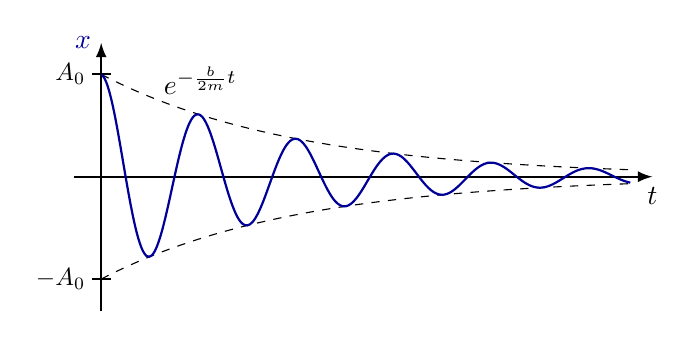
\begin{tikzpicture}
    \def\xmax{7.0} % max x axis
    \def\ymax{1.7}
    \def\A{1.3}
    \def\om{(5.3*360/(0.94*\xmax))}
    \def\t{1800/(0.94*\xmax)}
    \def\T{2.5}

    % AXIS
    \draw[->,thick] (0,-\ymax) -- (0,\ymax) node[left,xcol] {$x$};
    \draw[->,thick] (-0.2*\ymax,0) -- (\xmax,0) node[below] {$t$};
    \tick{0,\A}{0} node[left=-1,scale=0.9] {$A_0$};
    \tick{0,-\A}{0} node[left=-1,scale=0.9] {$-A_0$};

    % PLOT
    \draw[dashed,samples=\N,smooth,variable=\t,domain=0:0.96*\xmax]
    plot(\t,{\A*exp(-\t/\T)}) plot(\t,{-\A*exp(-\t/\T)});
    \draw[xline,samples=100+\N,smooth,variable=\t,domain=0:0.96*\xmax]
    plot(\t,{\A*exp(-\t/\T)*cos(\om*\t)});
    \node[above=4] at (0.18*\xmax,{\A*exp(-0.18*\xmax/\T)}) {$e^{-\frac{b}{2m}t}$};

\end{tikzpicture}

\end{document}